\documentclass[10pt]{article}

%defines page size and margins
\usepackage{geometry}
\geometry{
    letterpaper,
    left=1in,
    right=1in,
    top=1in,
    bottom=1in,
}

%Sets spacing for entire document
\usepackage{setspace}
\singlespacing

%Package for reducing space in between list items
\usepackage{enumitem}

%Math symbols
\usepackage{gensymb}

%Image path
\usepackage{graphicx}
\graphicspath{ {/} }

%Used for adjusting images
\usepackage[export]{adjustbox}

%For floating images
\usepackage{float}

\begin{document}
\title{Laboratory One --- Circuit Simulation With Spice}
\date{September 29, 2017}
\author{Rishabh Shah\\ Partner: Matthew Remillard}
\maketitle

\section*{Pre-Lab}
\begin{figure}[H]
	\centering
		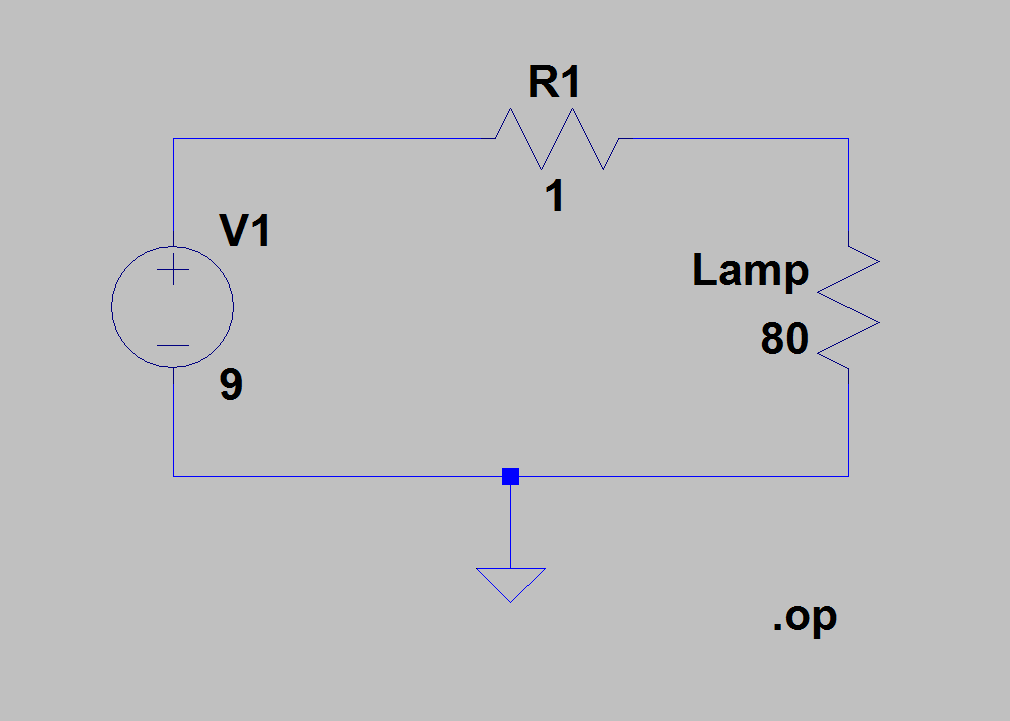
\includegraphics[width=5in]{Capture1}
	\caption{Lamp circuit schematic.}
\end{figure}
\begin{figure}[H]
	\centering
		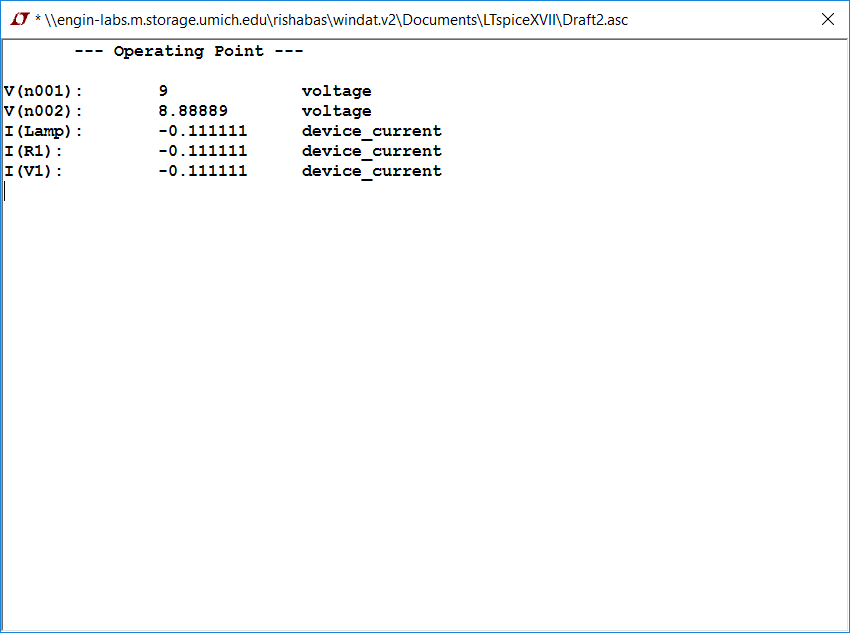
\includegraphics[width=5in]{Capture}
	\caption{Element and node values for the lamp circuit.}
\end{figure}
\begin{figure}[H]
	\centering
		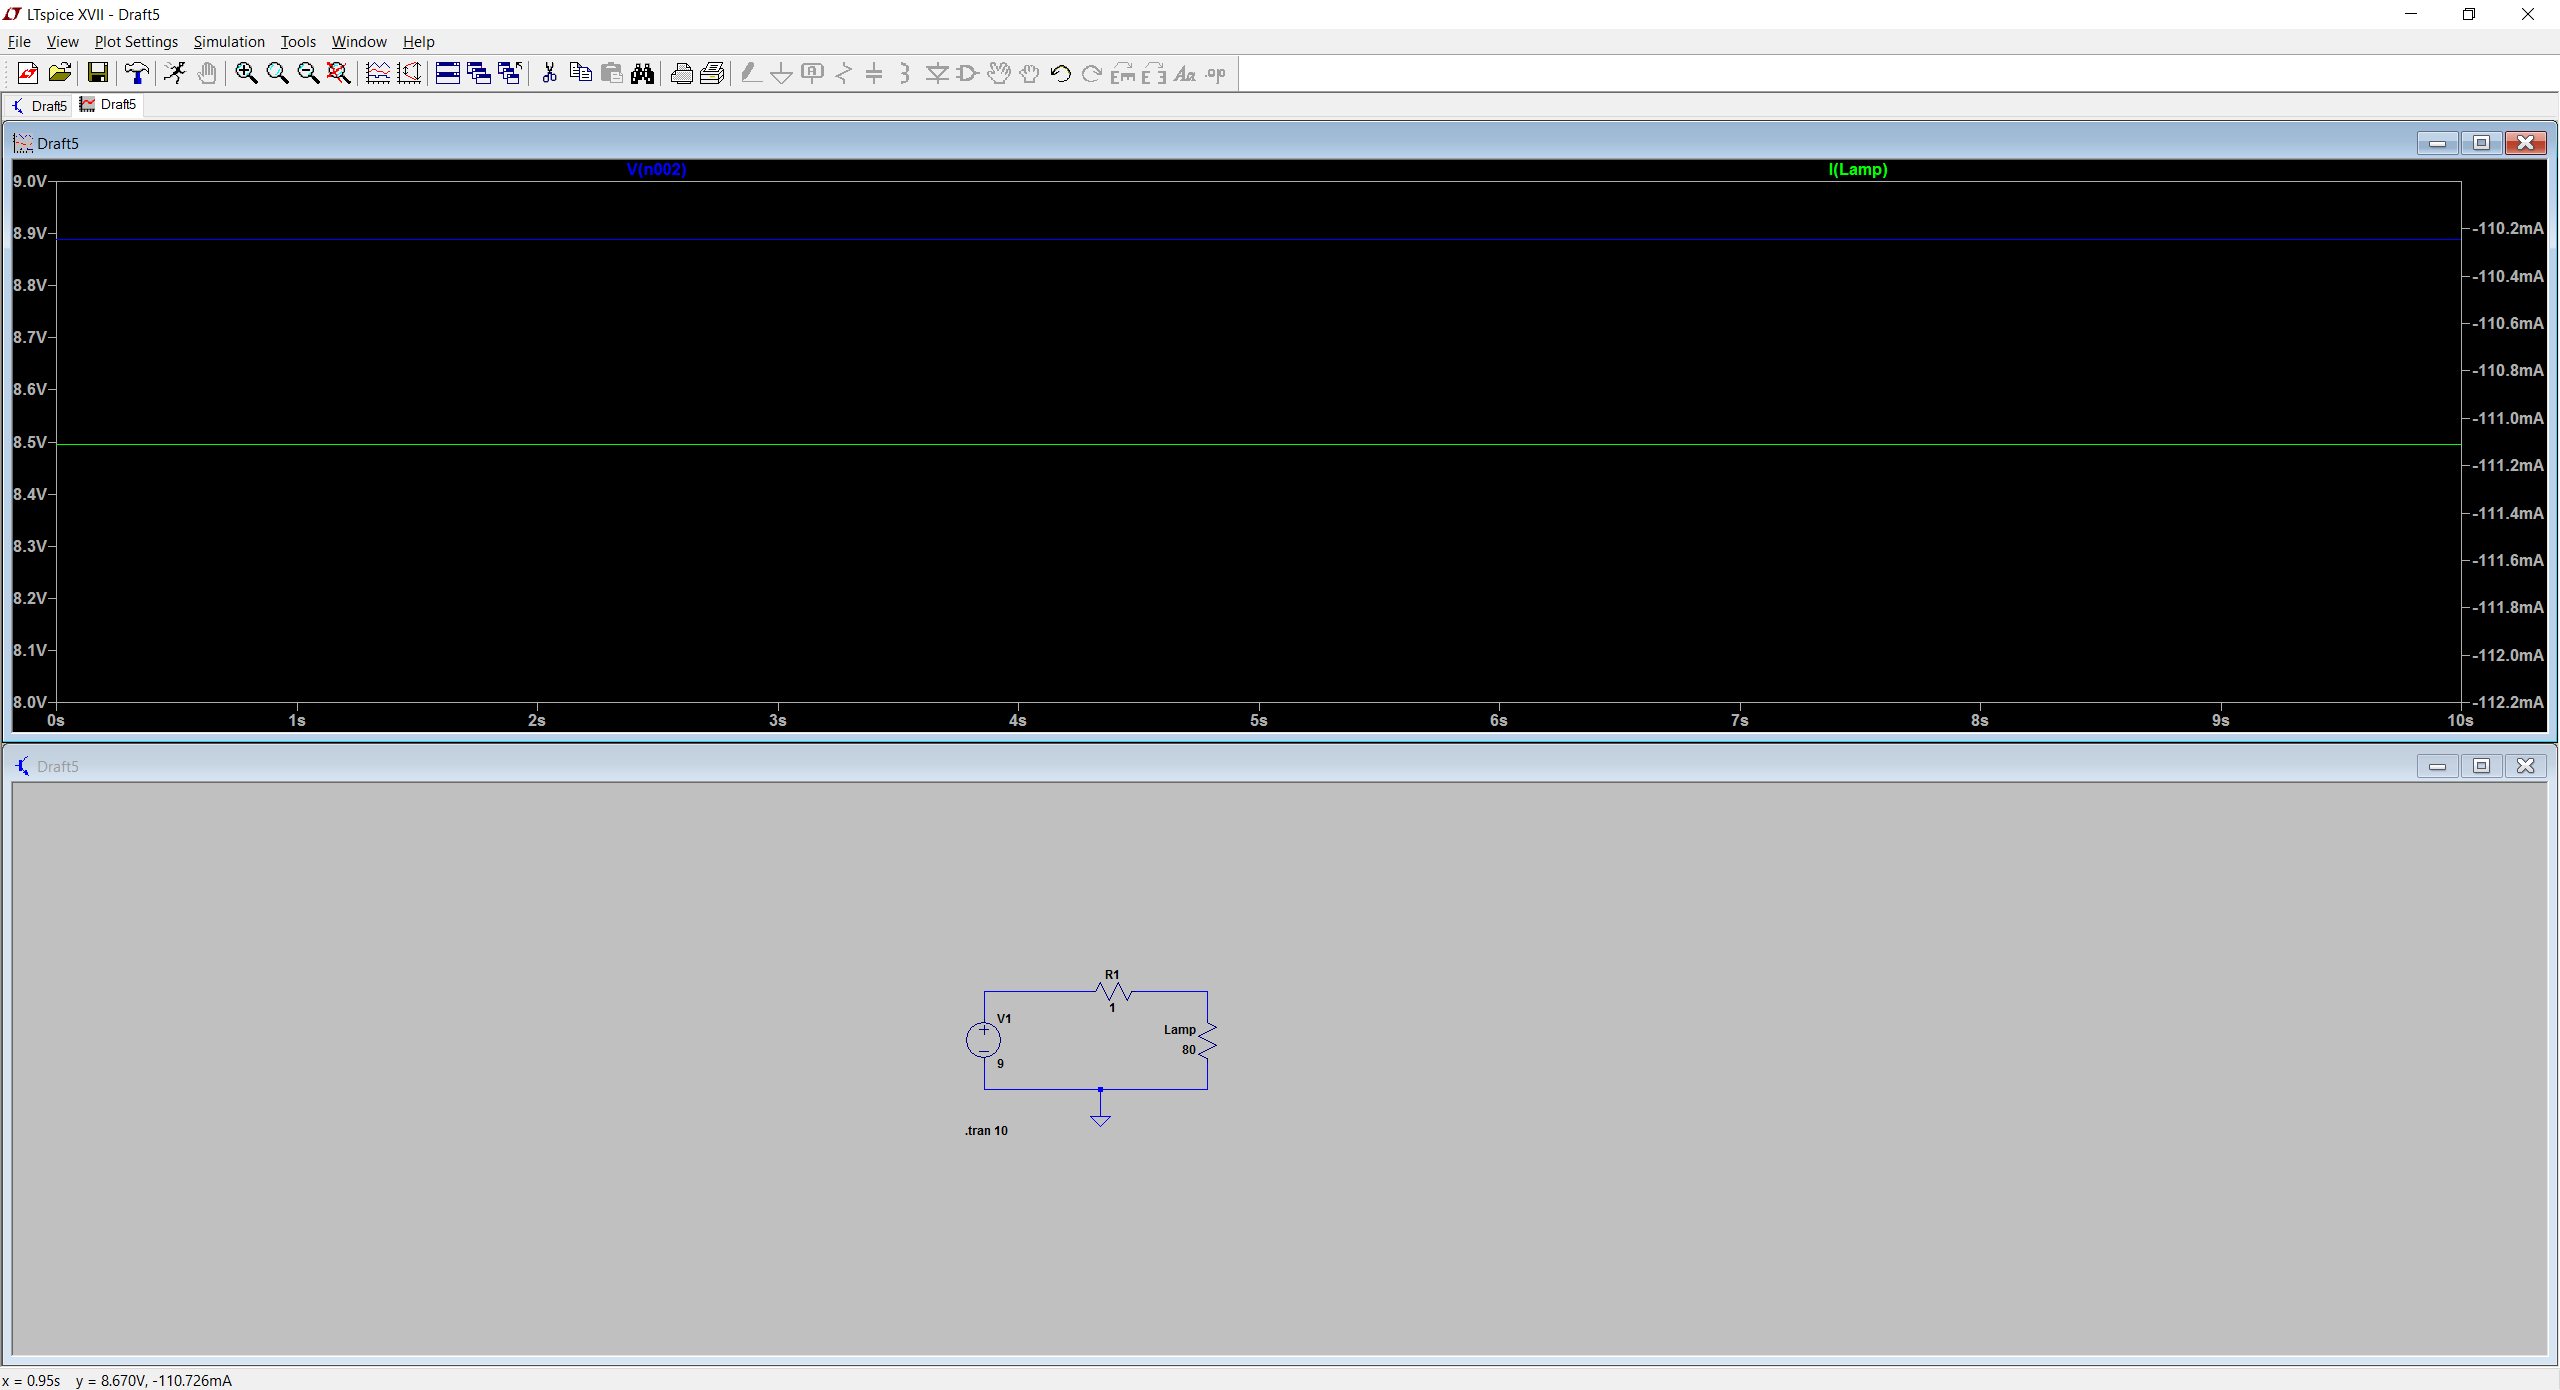
\includegraphics[width=5in]{Capture10}
	\caption{Graph of current through and voltage drop across the light bulb in the lamp circuit.}
\end{figure}

\section*{Post-Lab}

\subsection*{Dependent Source Circuit}
\begin{figure}[H]
	\centering
		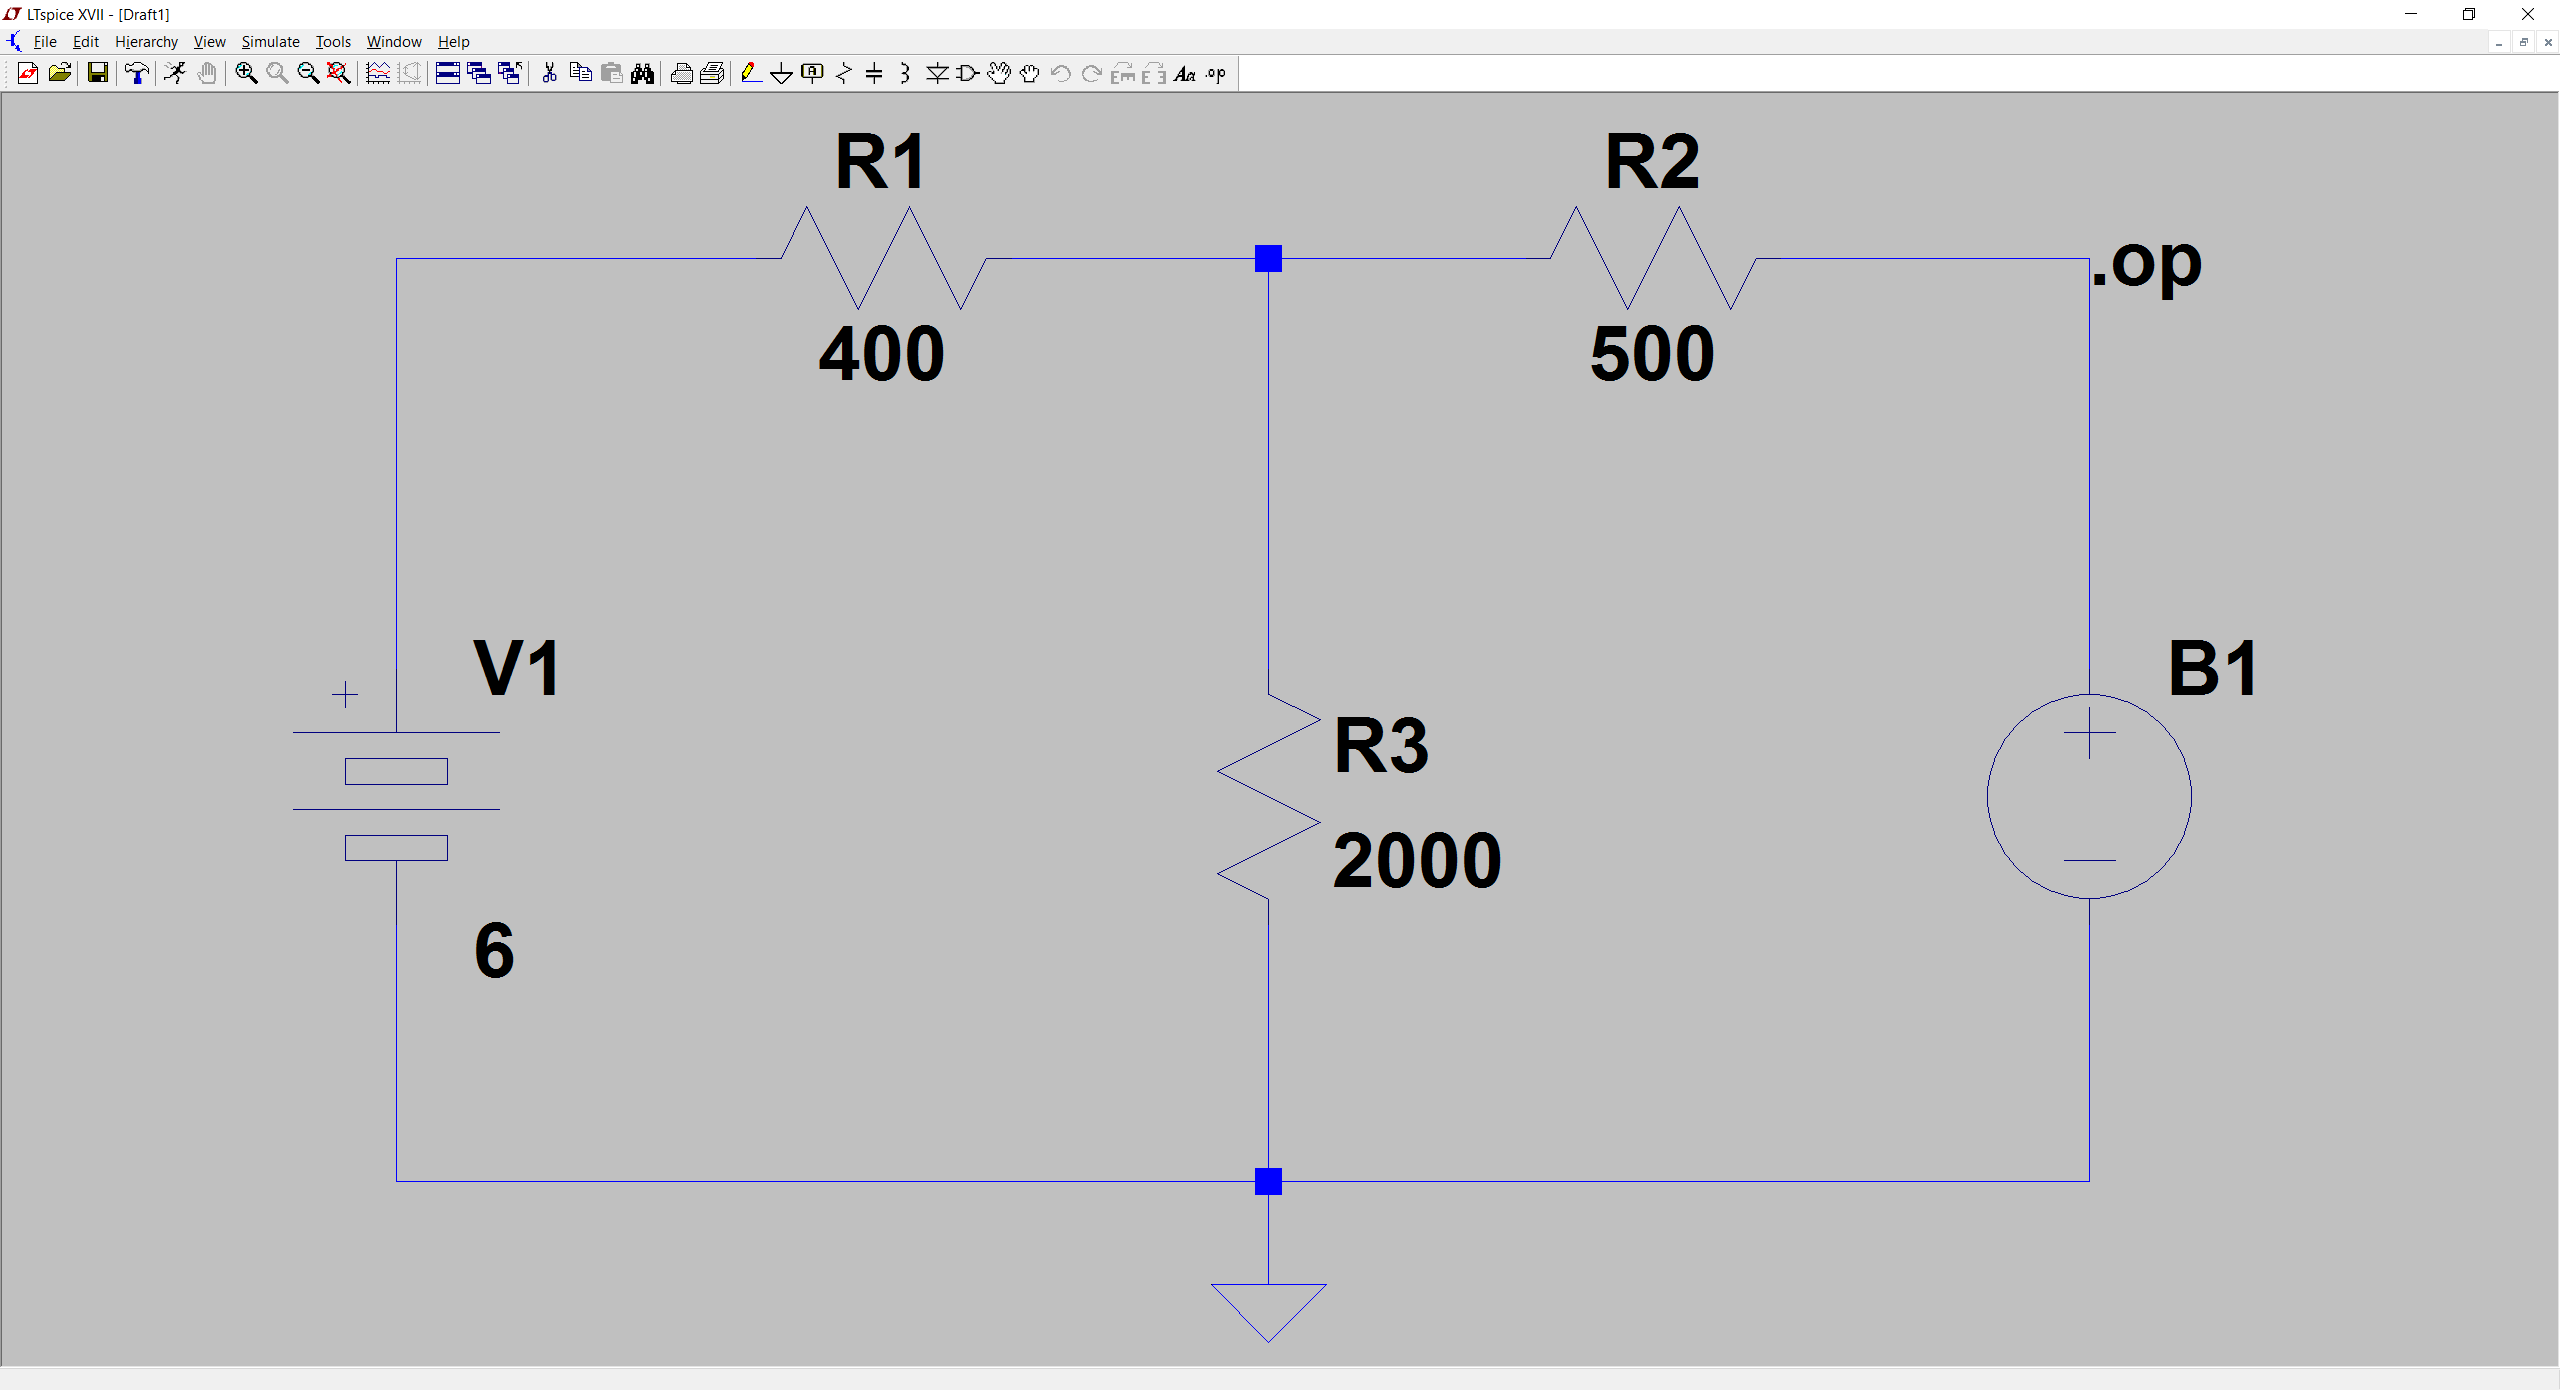
\includegraphics[width=5in]{Capture2}
	\caption{Dependent source circuit schematic.}
\end{figure}
\begin{figure}[H]
	\centering
		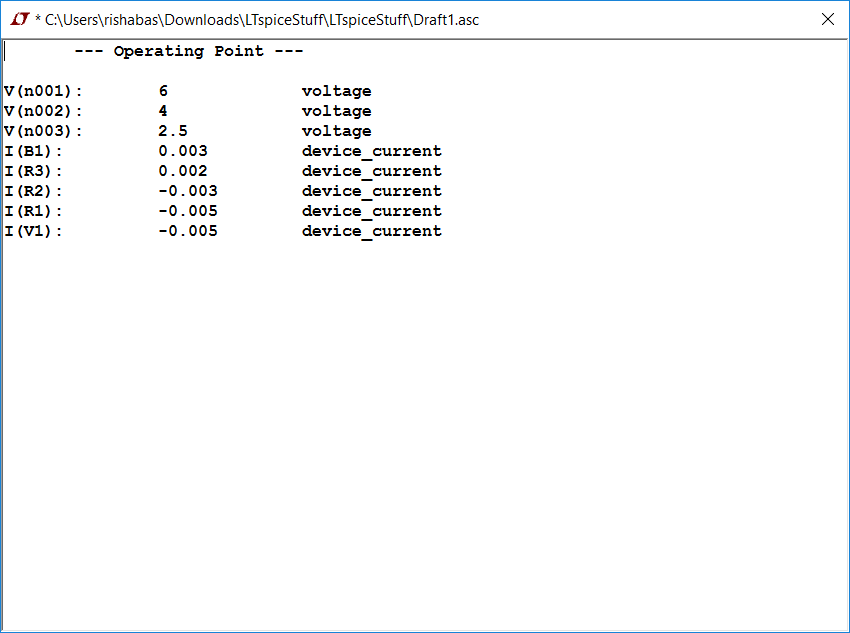
\includegraphics[width=5in]{Capture3}
	\caption{Element and node voltages for dependent source circuit.}
\end{figure}
\begin{figure}[H]
	\centering
		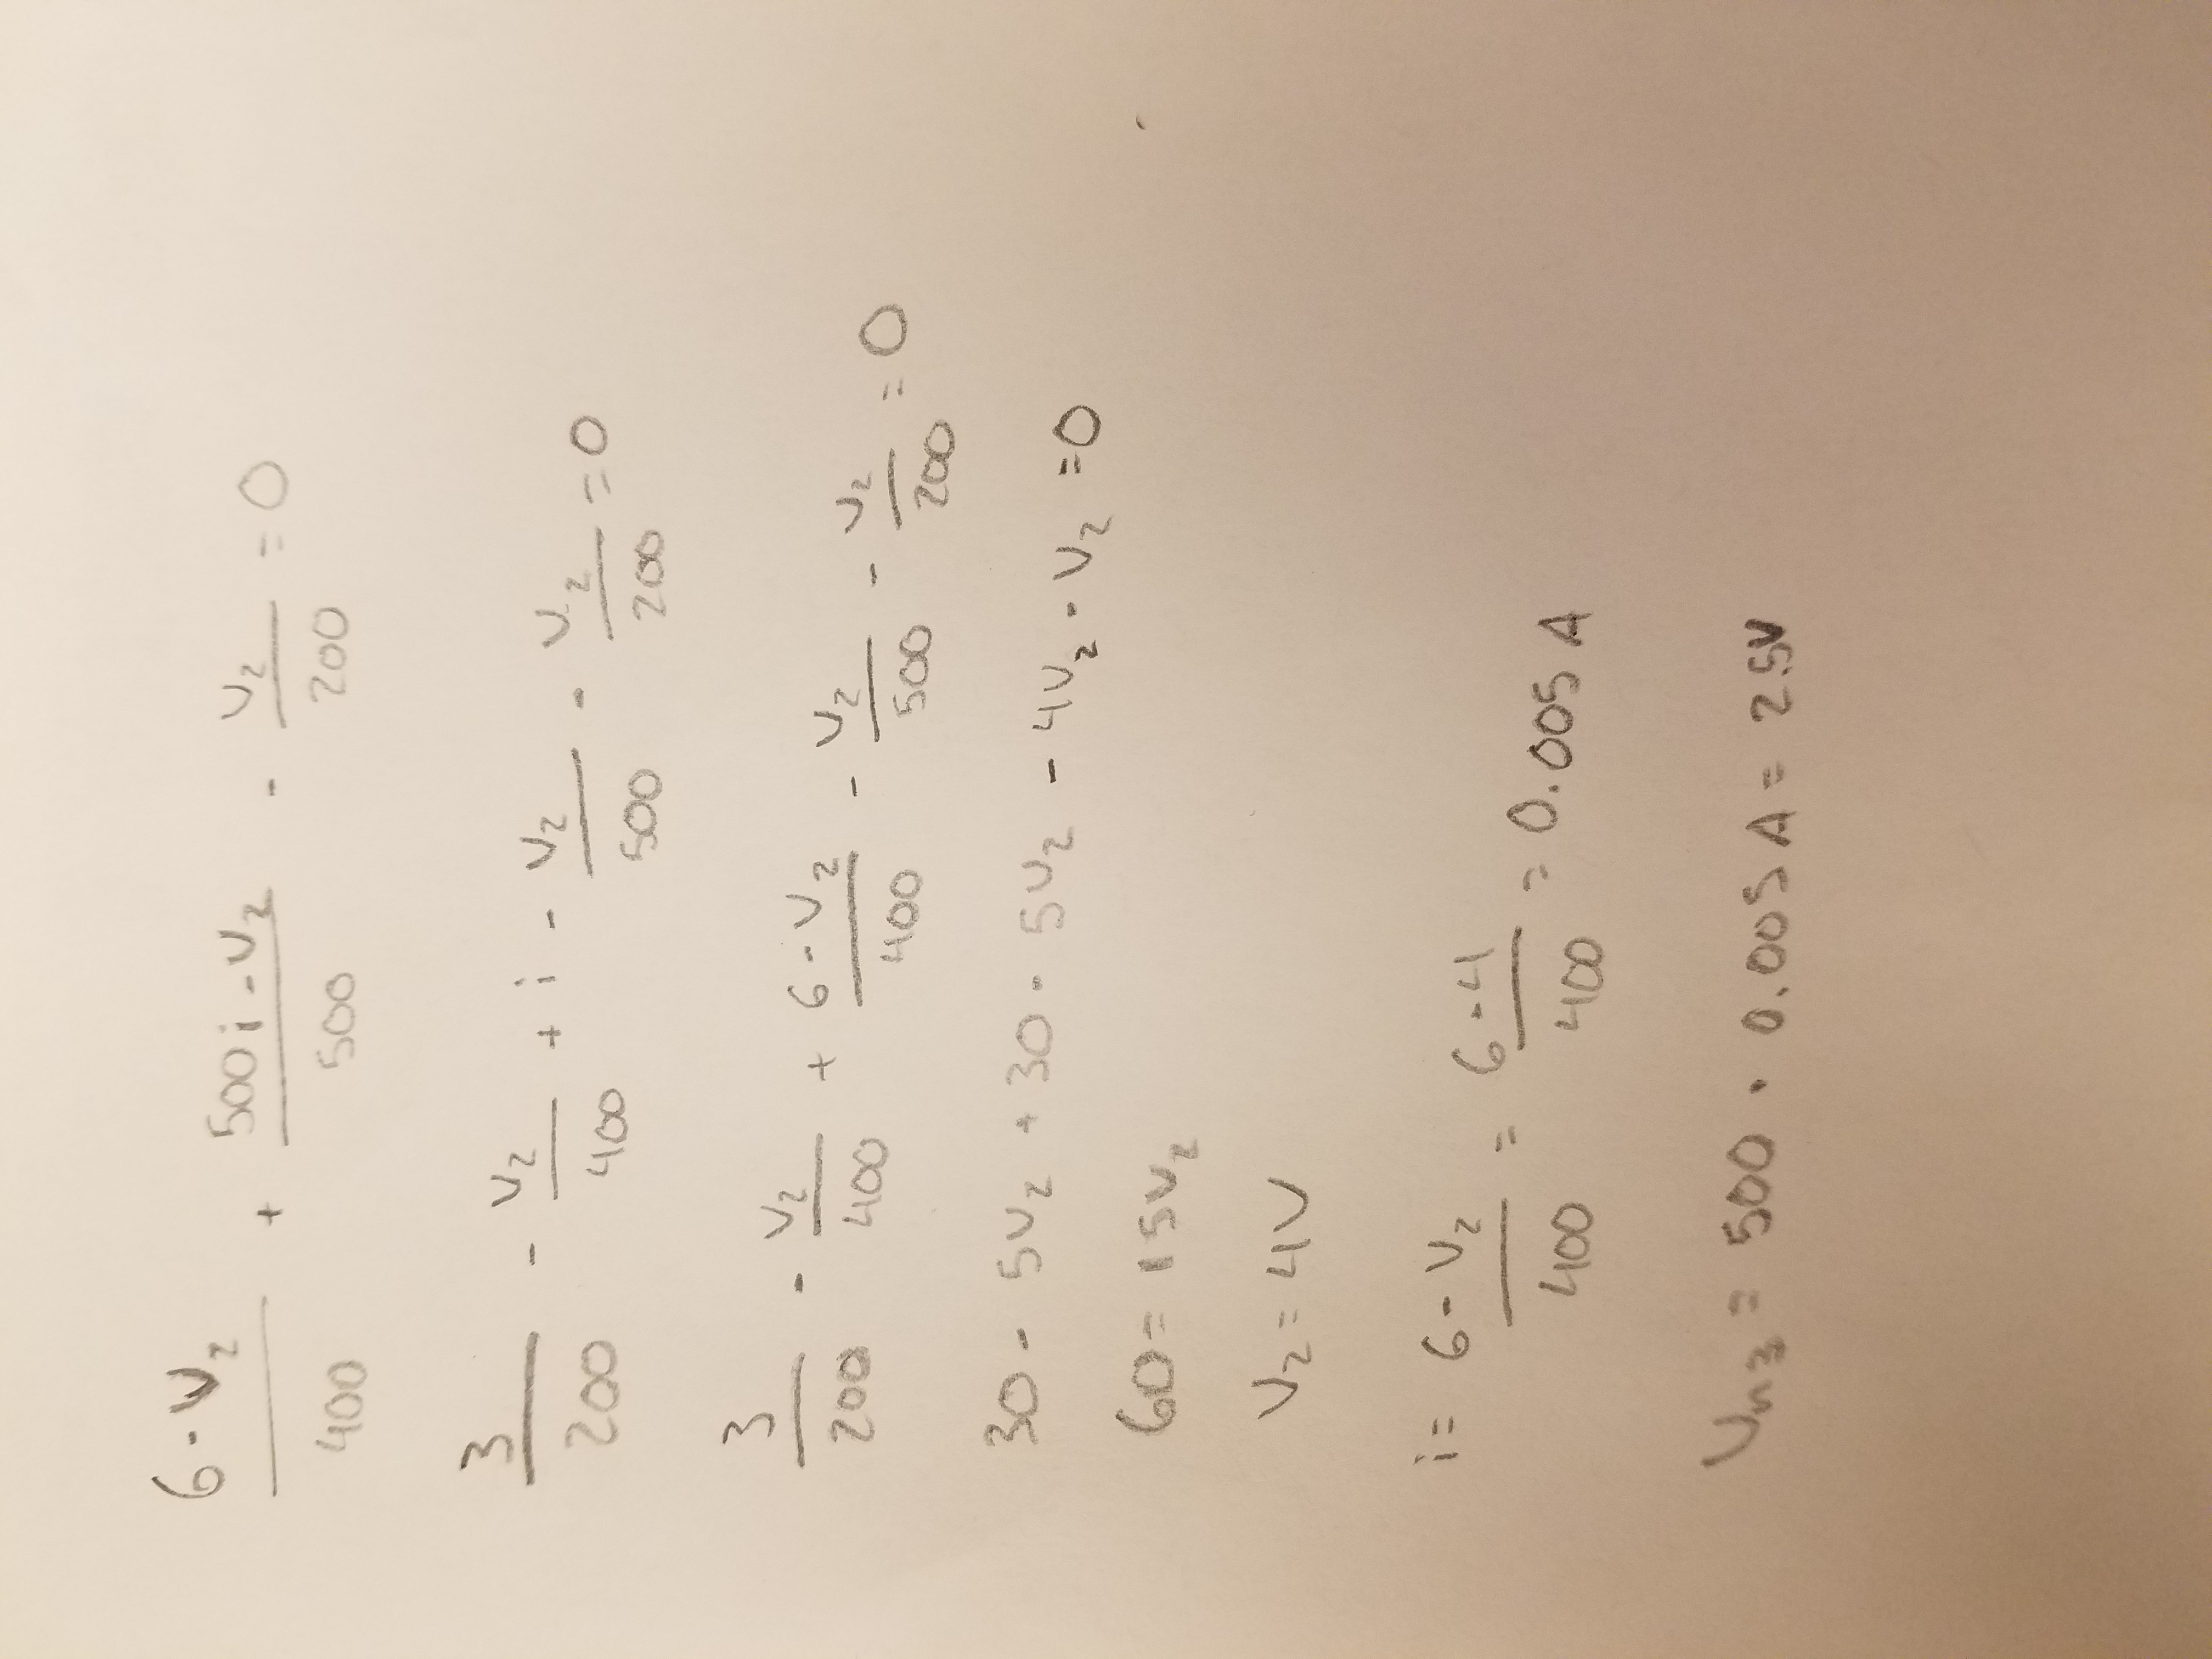
\includegraphics[width=5in, angle=270]{Capture11}
	\caption{Nodal analysis by hand for the dependent source circuit.}
\end{figure}

\subsection*{Lamp Circuit}
\begin{figure}[H]
	\centering
		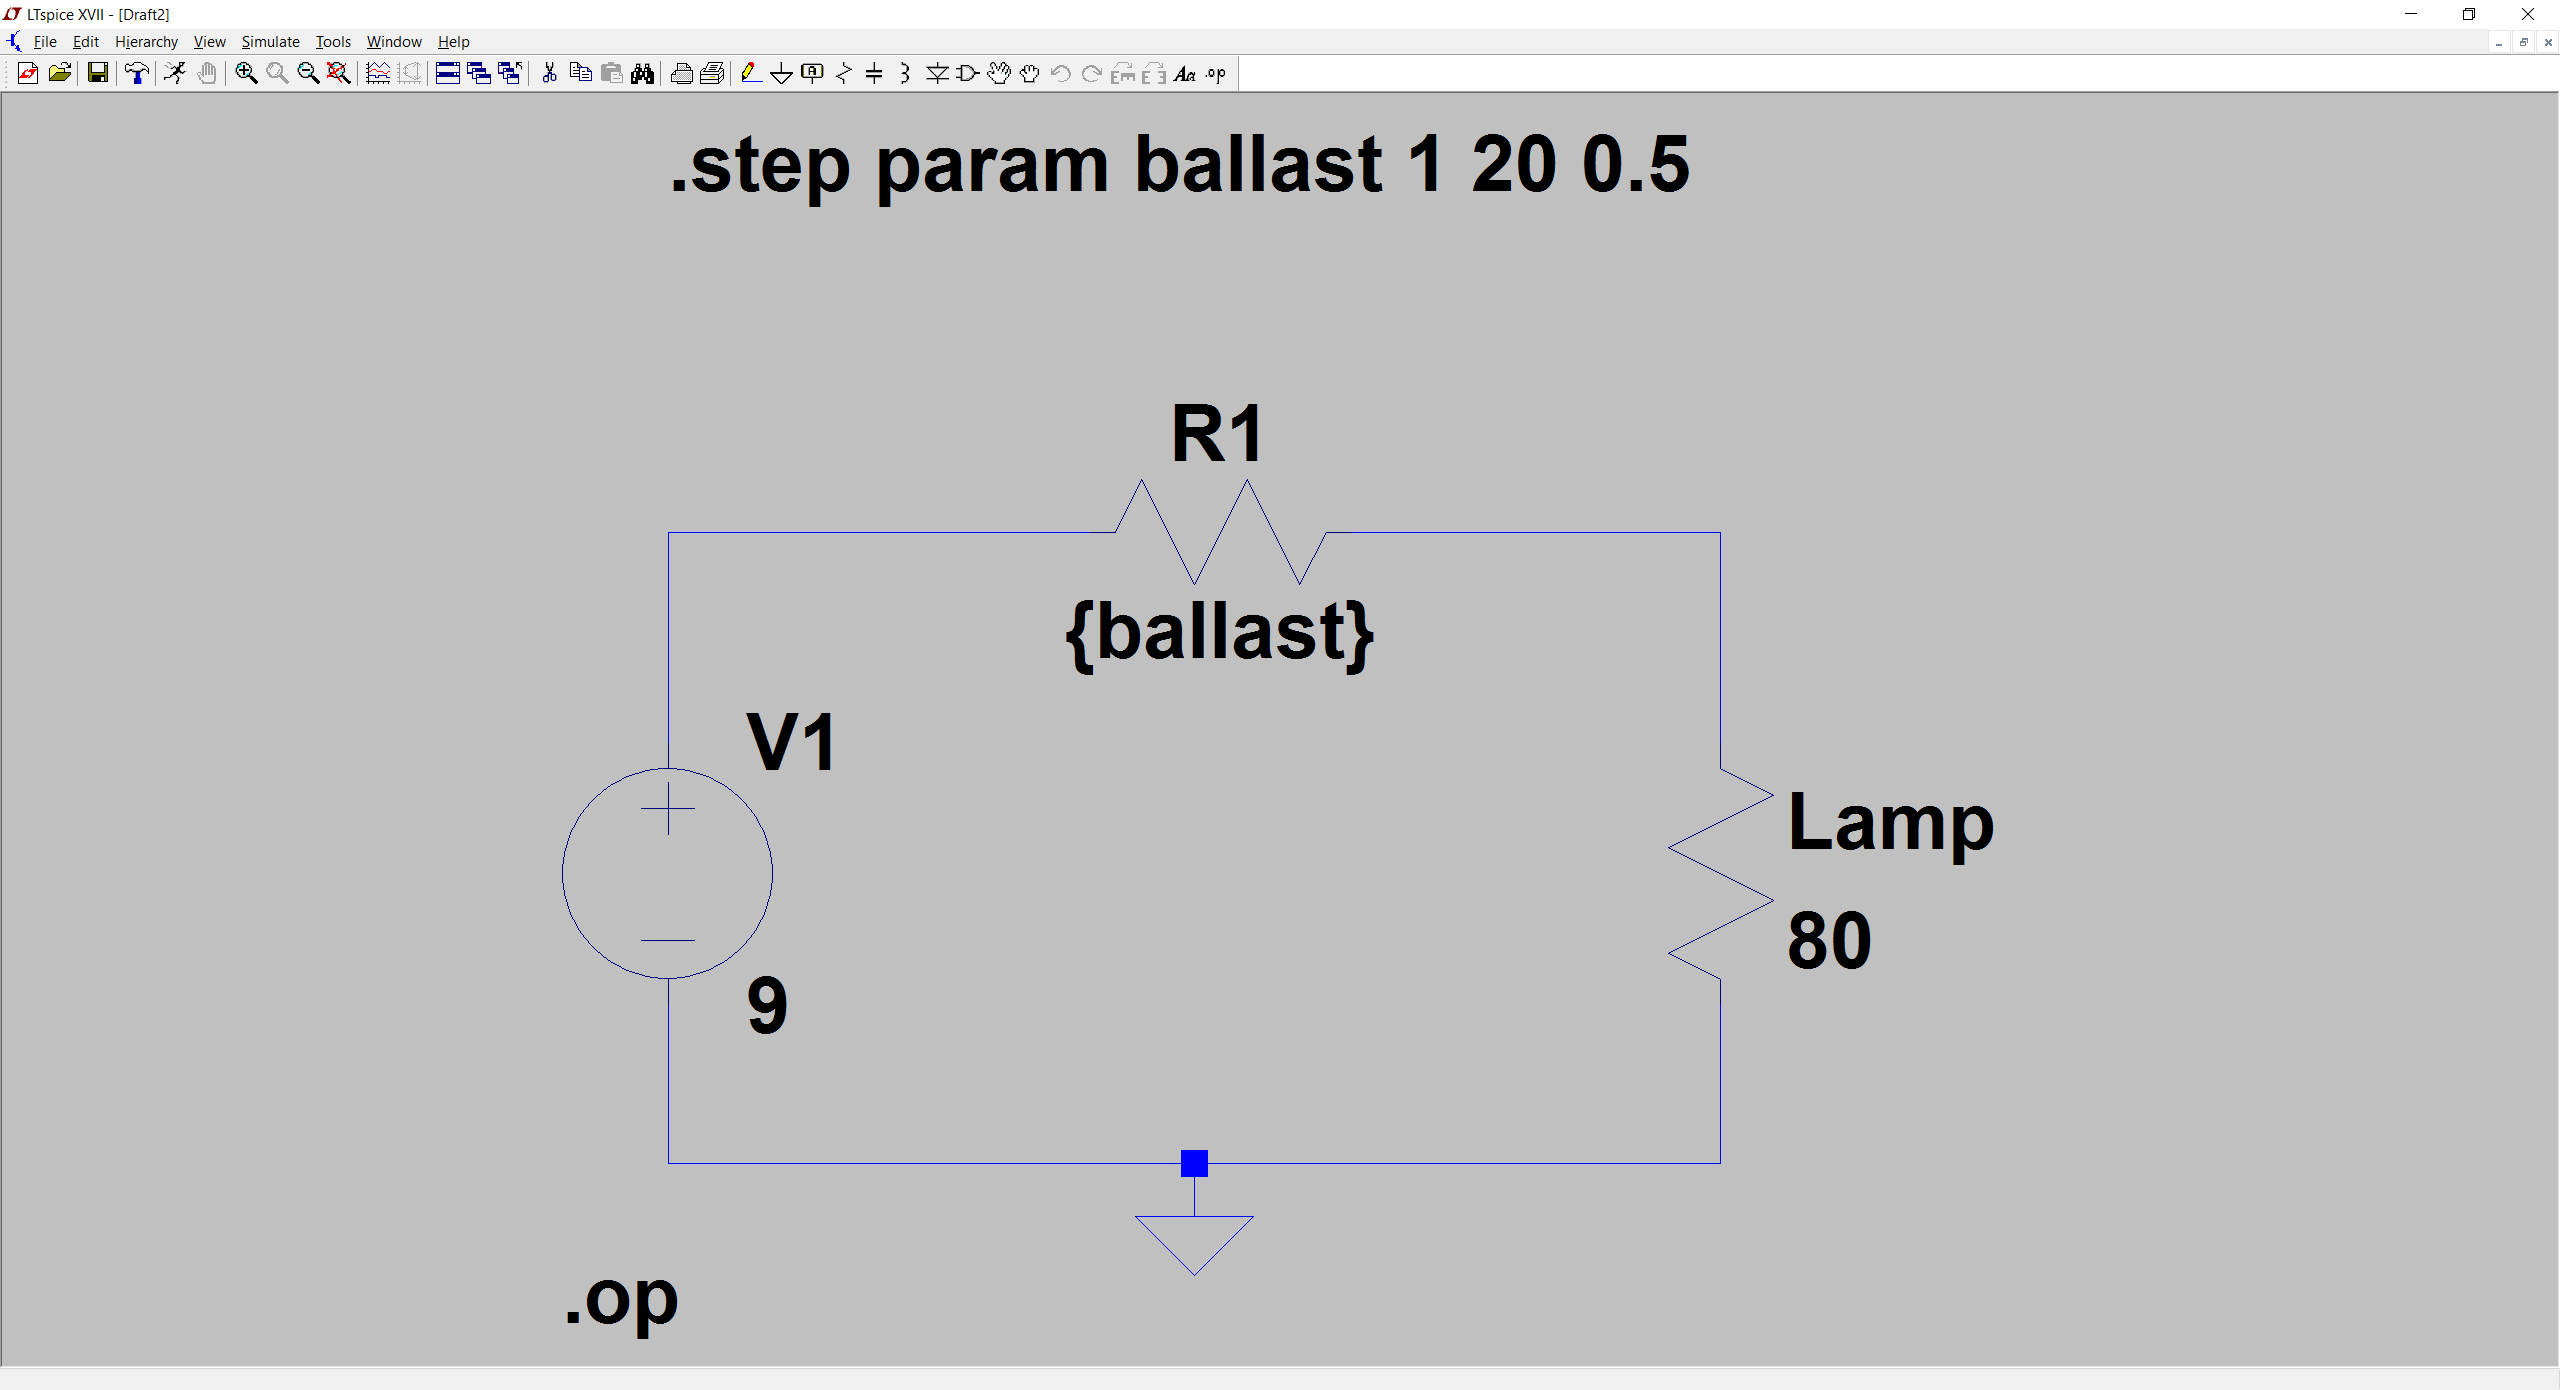
\includegraphics[width=5in]{Capture4}
	\caption{Lamp circuit with ballast schematic.}
\end{figure}
\begin{figure}[H]
	\centering
		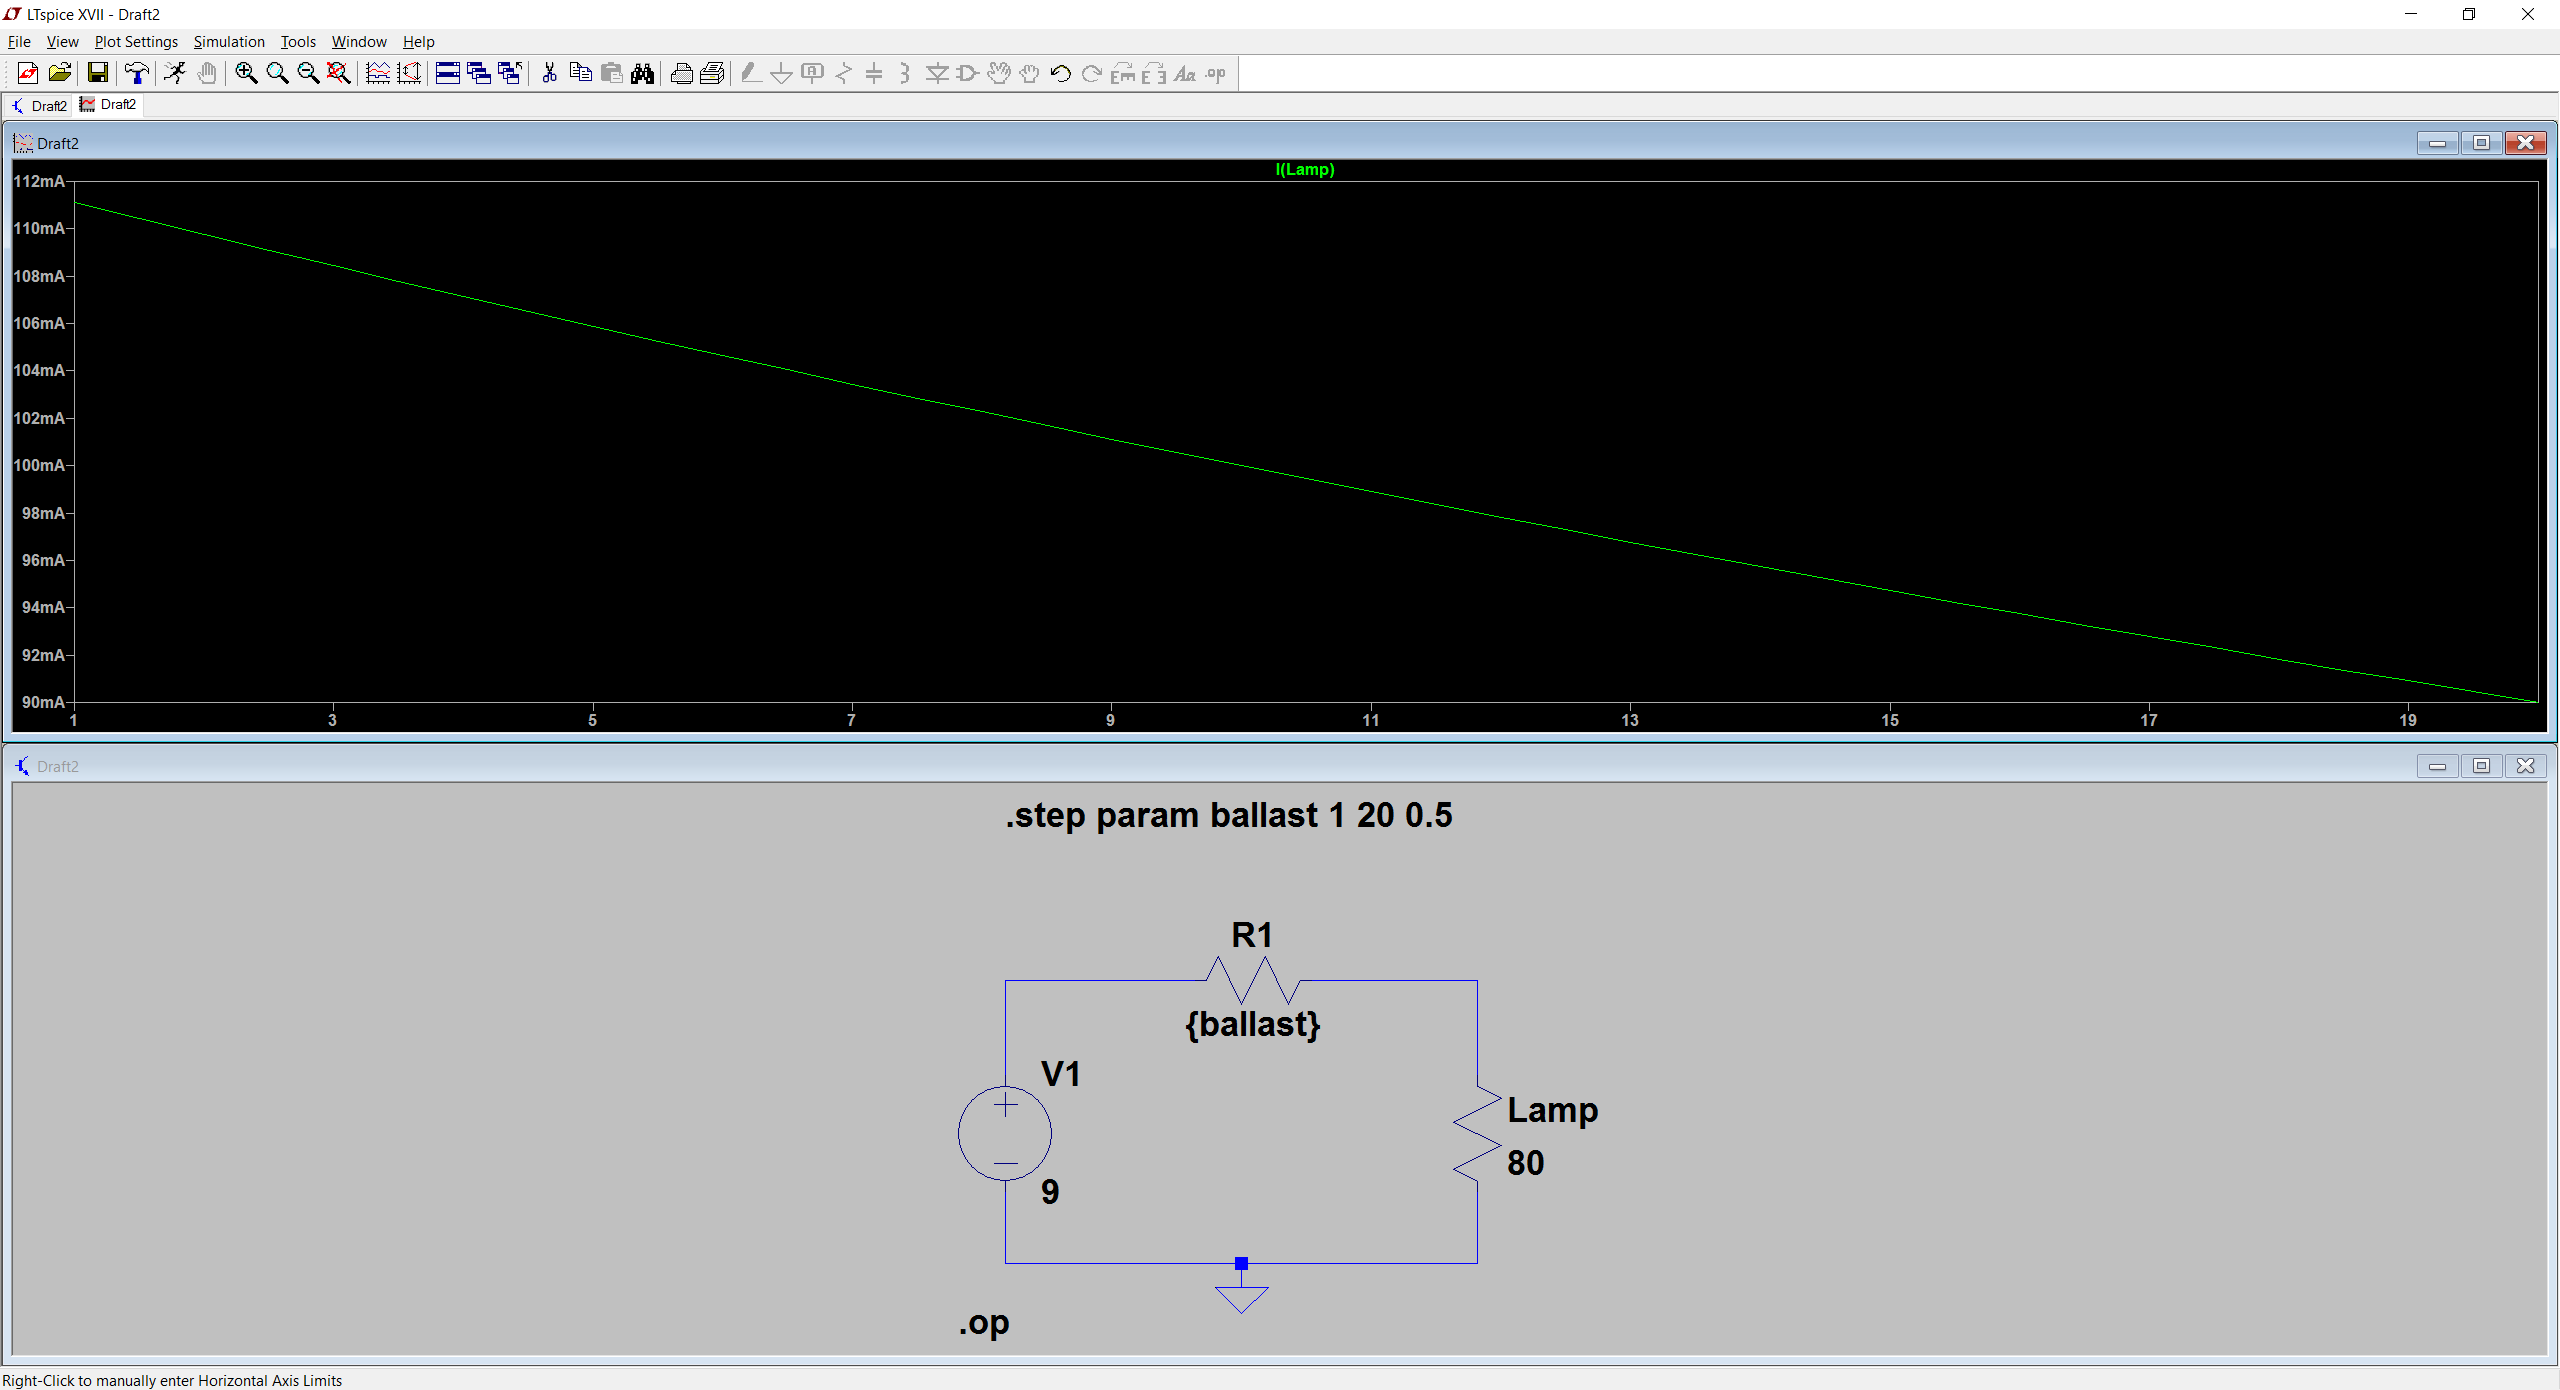
\includegraphics[width=5in]{Capture5}
	\caption{Lamp circuit graph of current vs. resistance.}
\end{figure}

\subsection*{LED Circuit}
\begin{figure}[H]
	\centering
		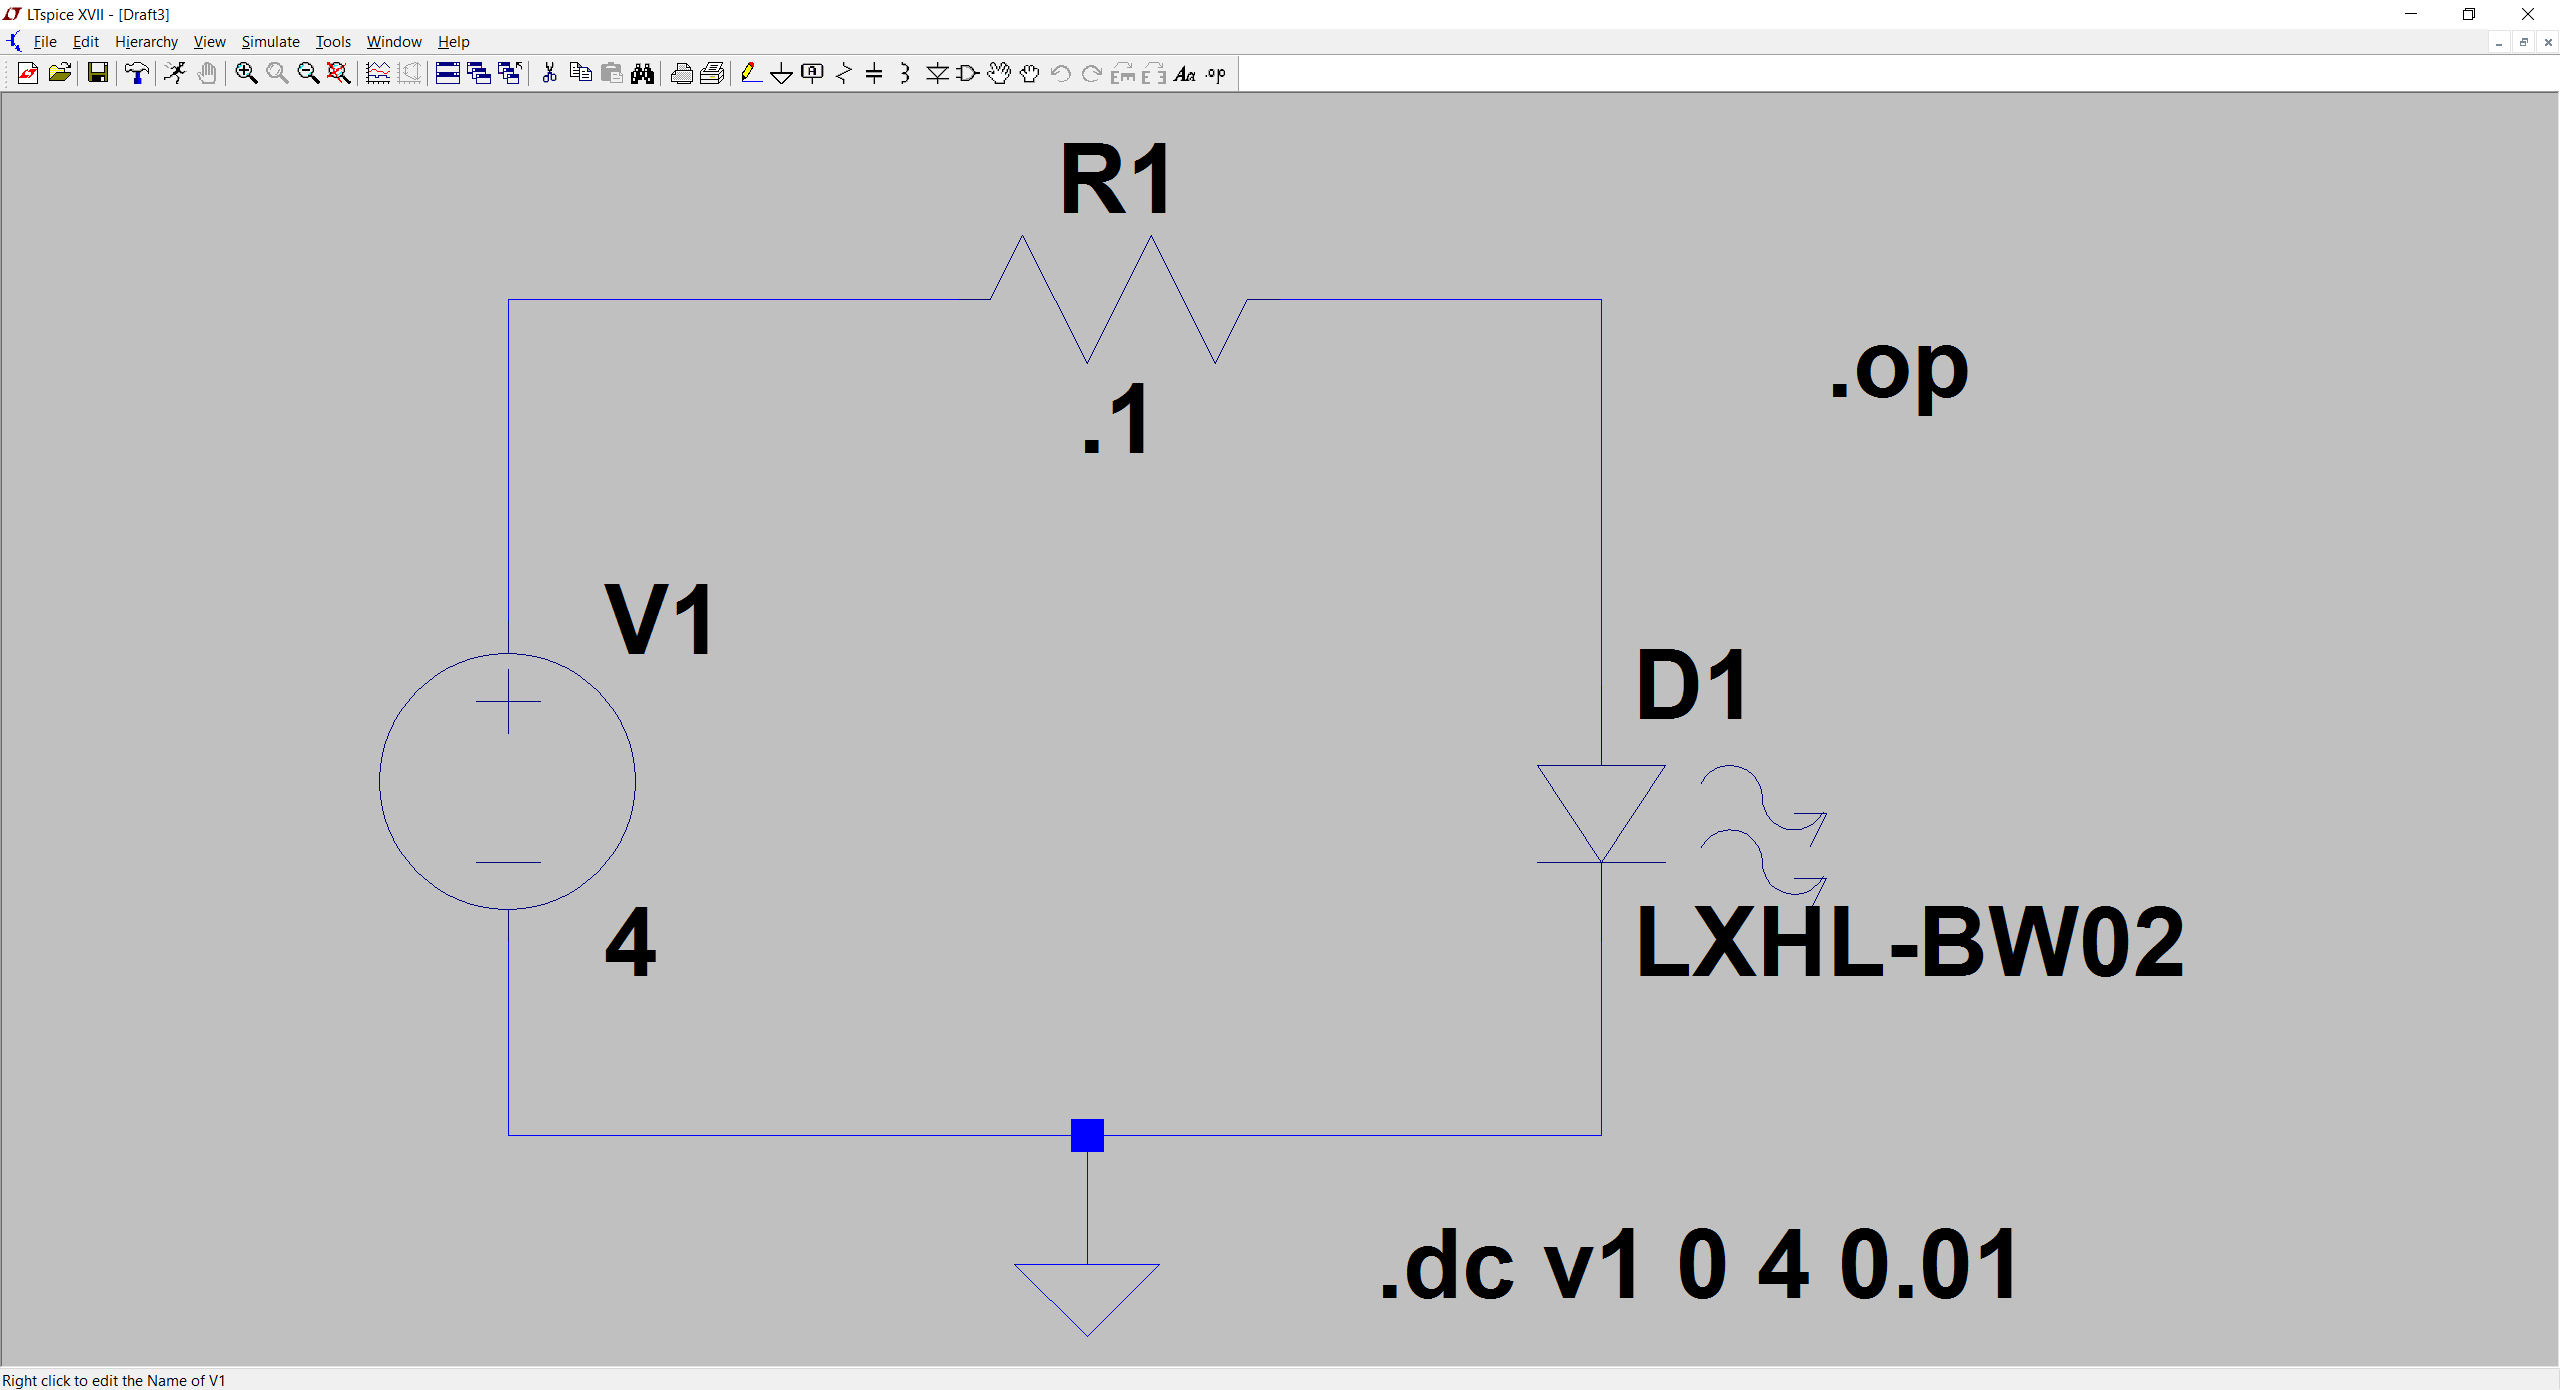
\includegraphics[width=5in]{Capture6}
	\caption{LED circuit schematic.}
\end{figure}
\begin{figure}[H]
	\centering
		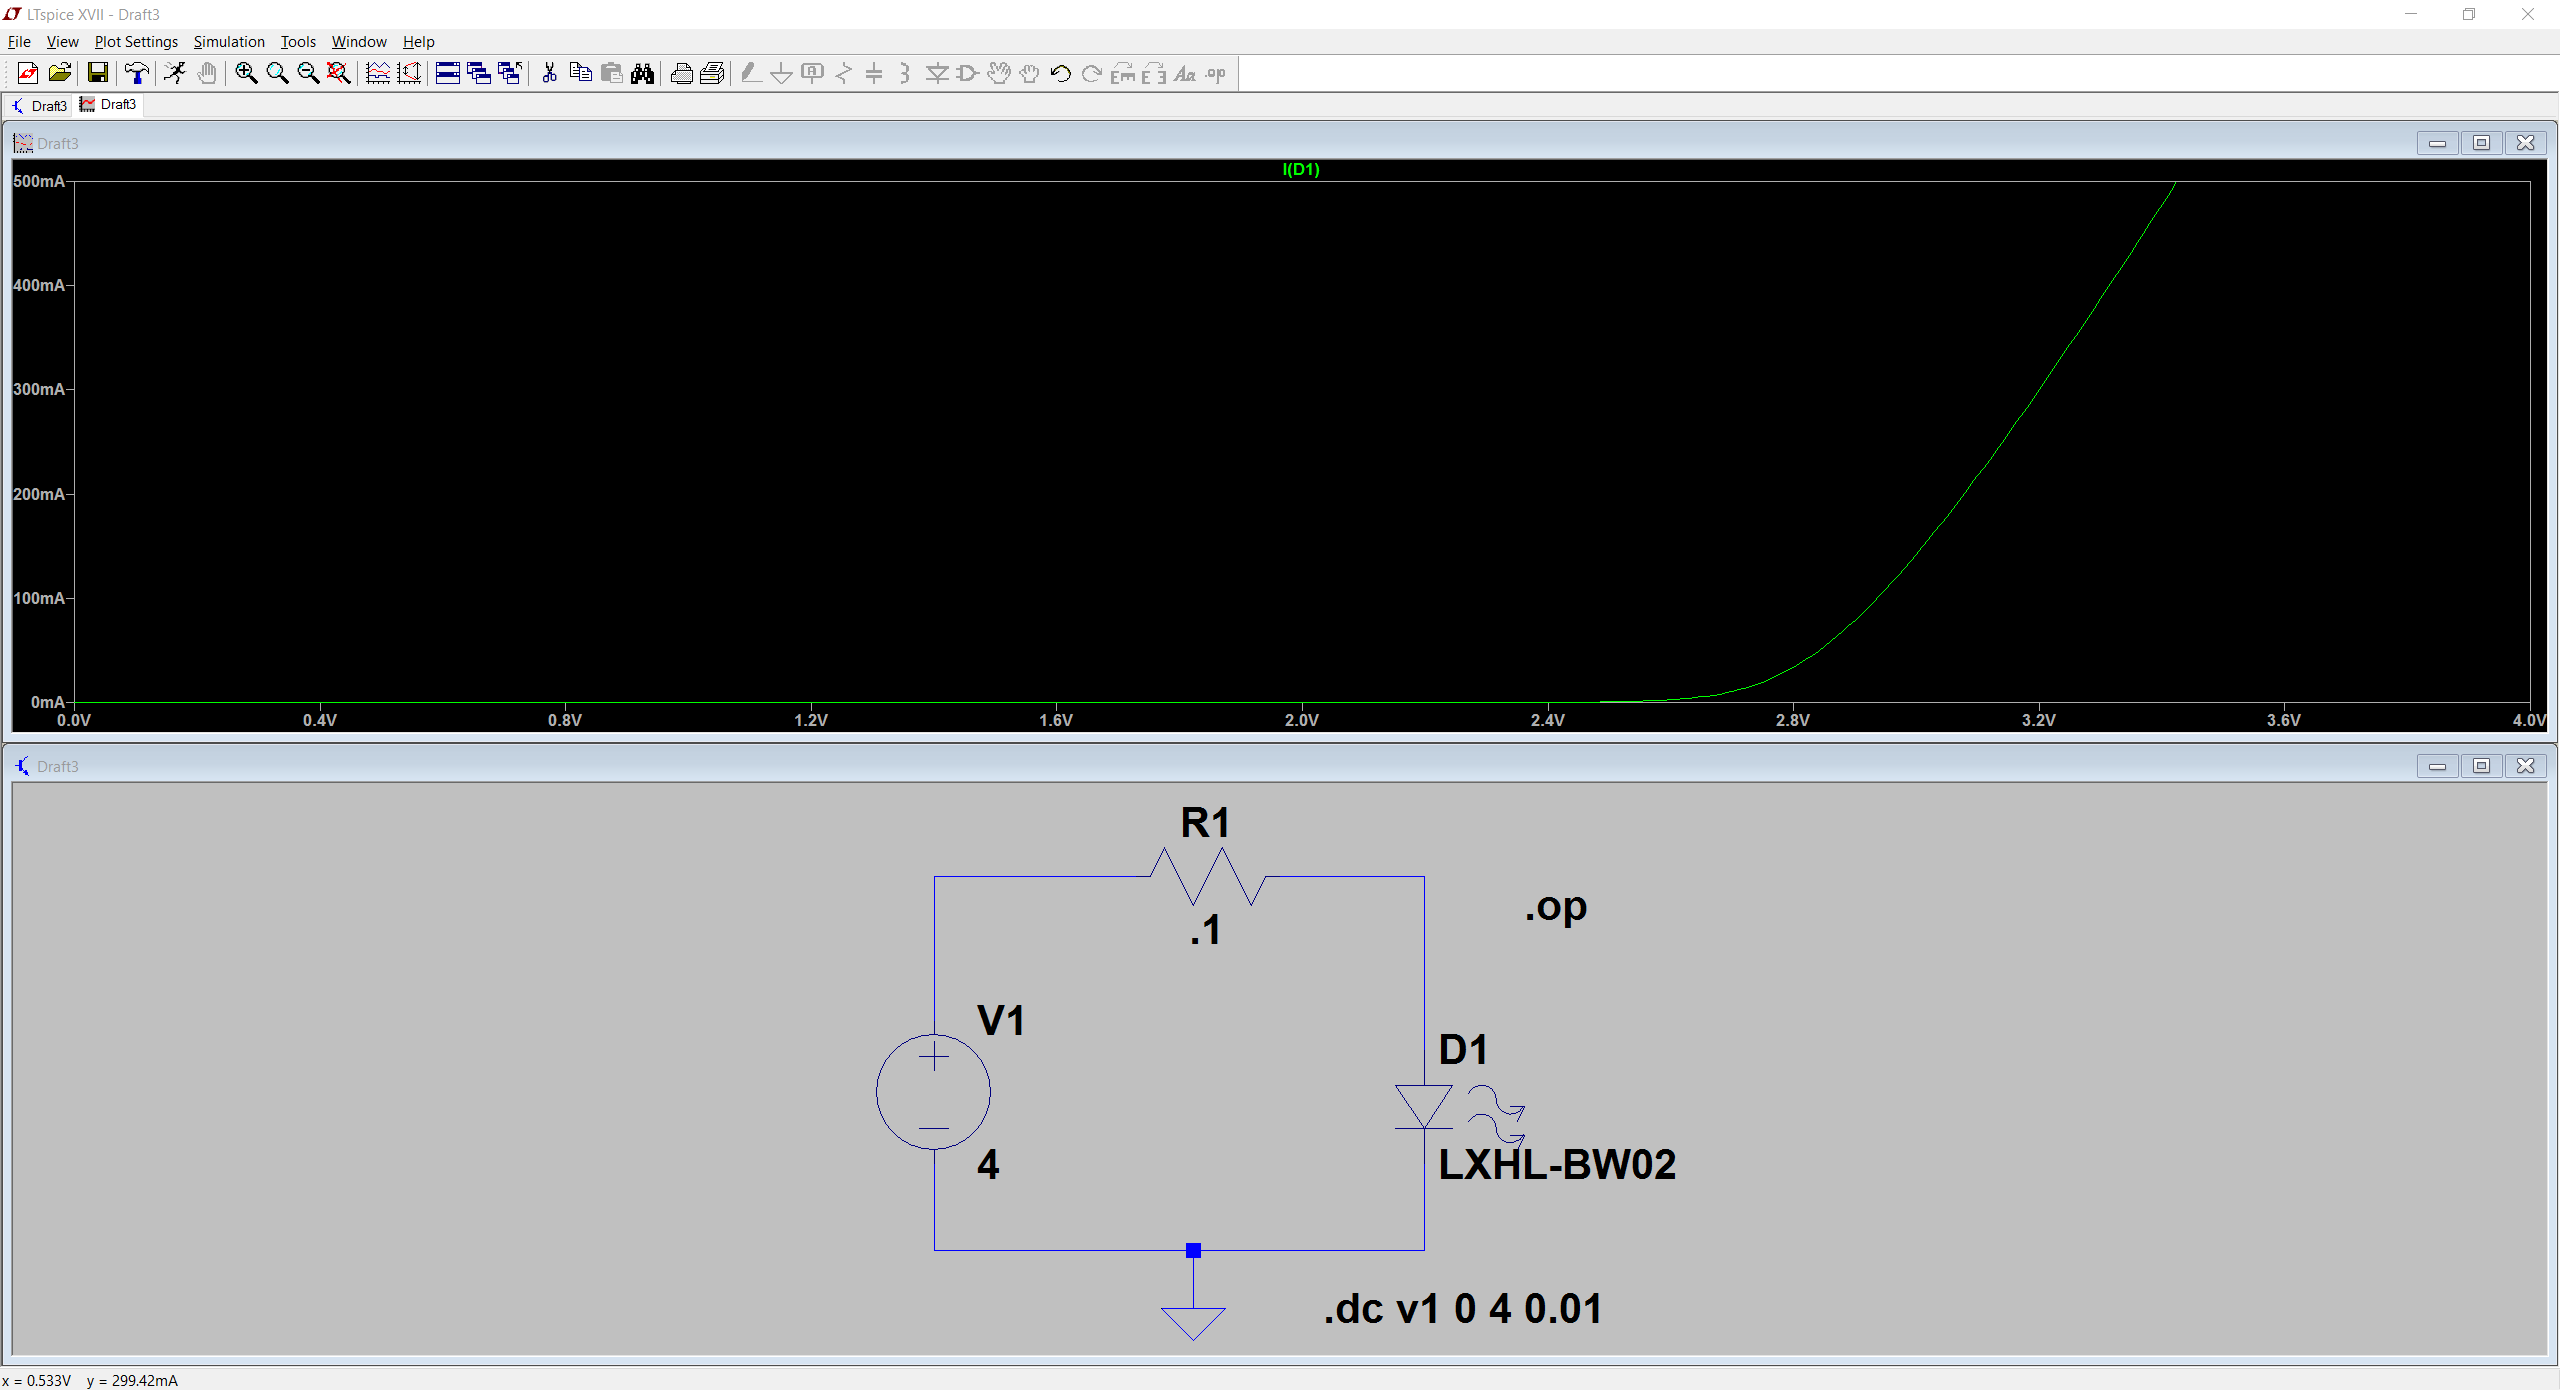
\includegraphics[width=5in]{Capture7}
	\caption{LED circuit graph of current vs. voltage.}
\end{figure}
\begin{figure}[H]
	\centering
		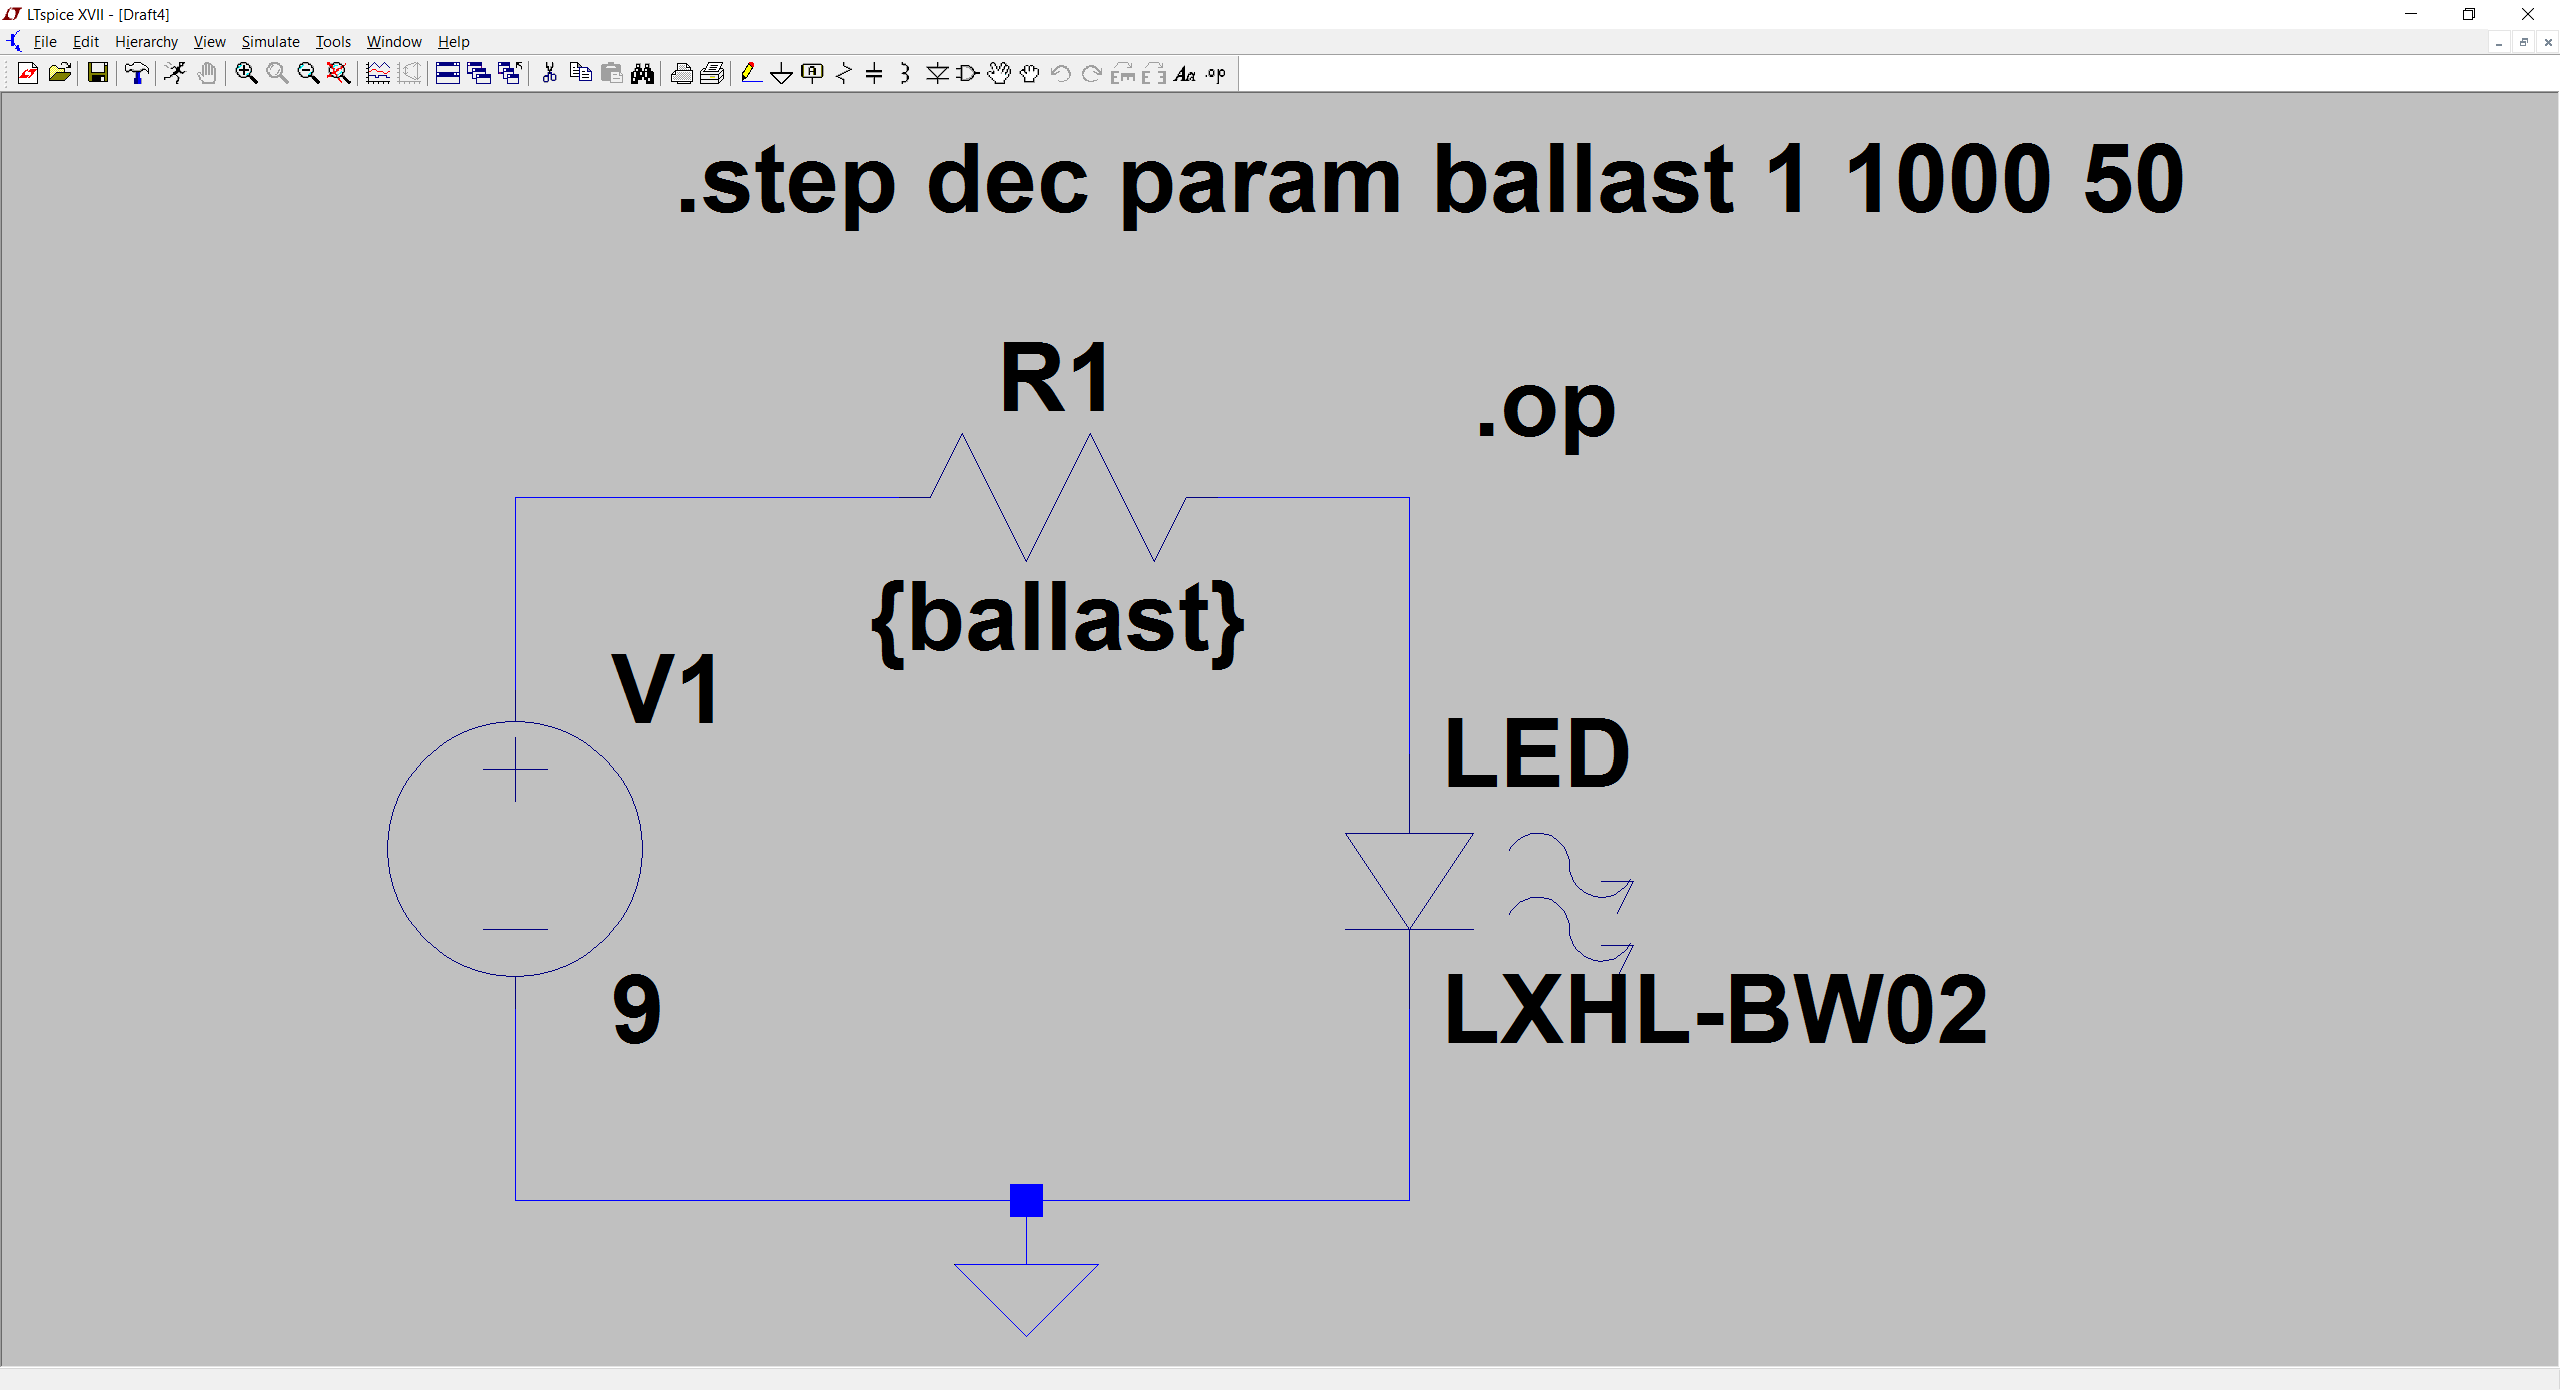
\includegraphics[width=5in]{Capture8}
	\caption{LED circuit with ballast schematic.}
\end{figure}
\begin{figure}[H]
	\centering
		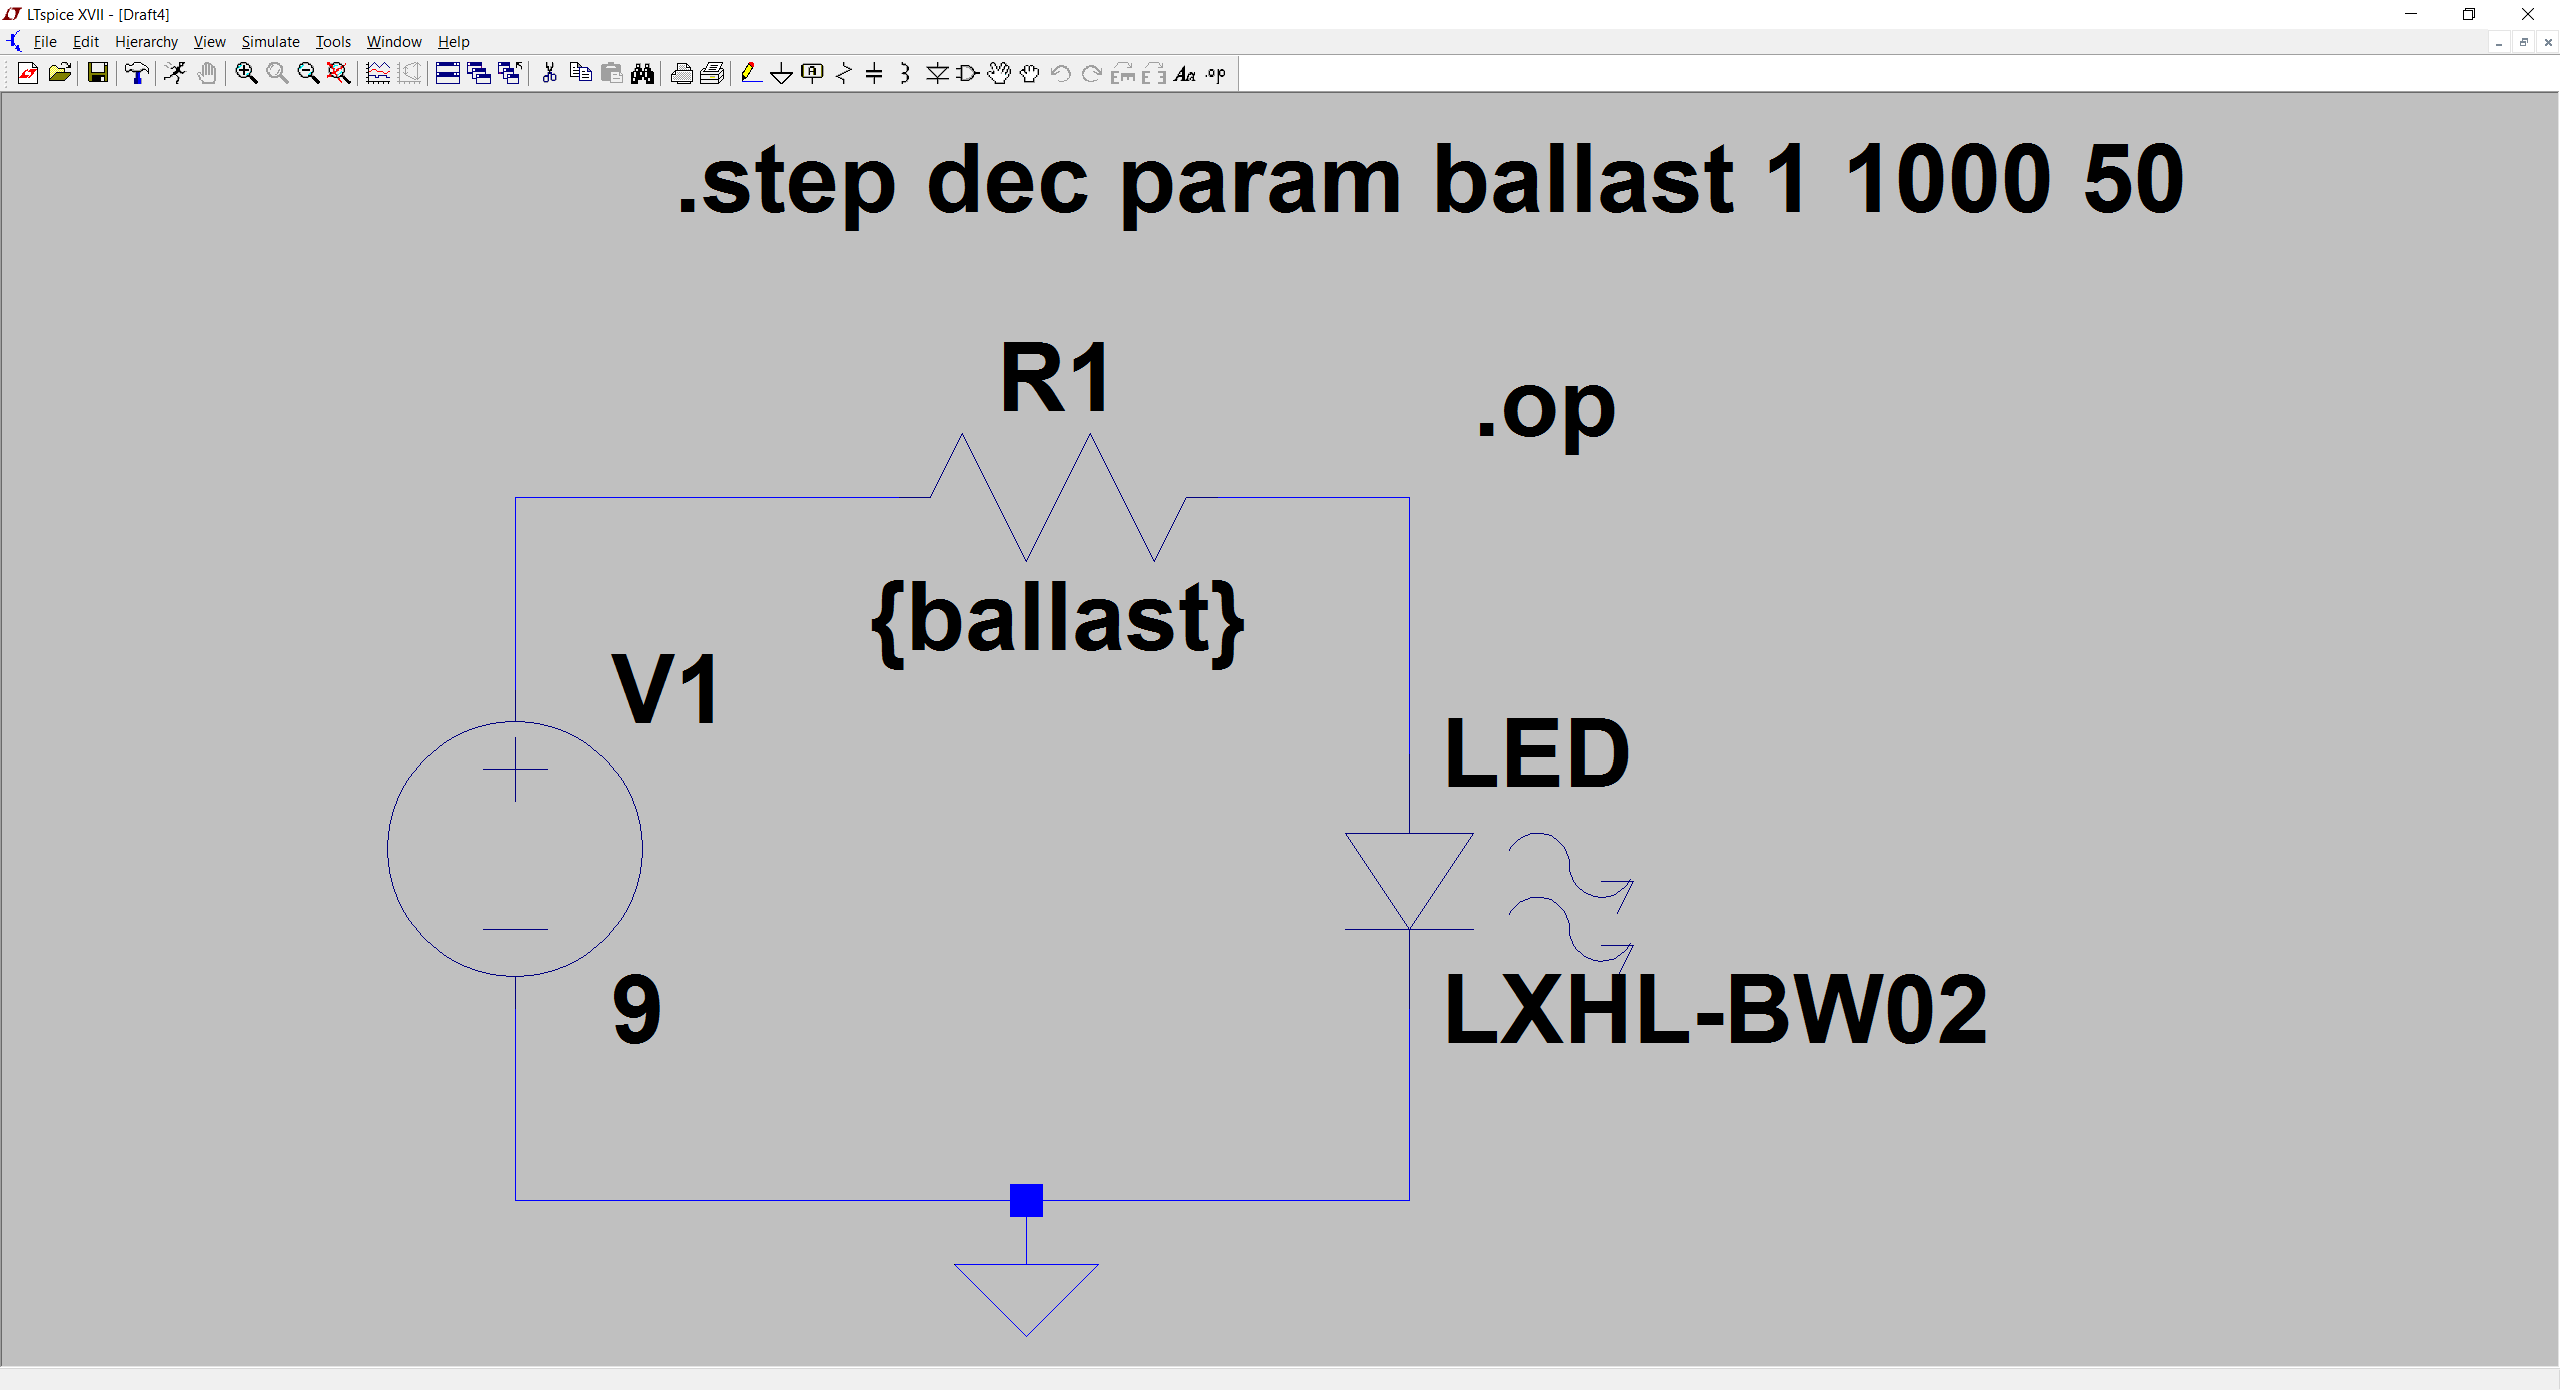
\includegraphics[width=5in]{Capture8}
	\caption{Graph of power consumption/absortion vs. resistance.}
\end{figure}

\end{document}
